\documentclass[text.tex]{subfiles}

\begin{document}

\section{Quasicrystal}\label{sec_quasicrystalEaseIn}%---------------------------------------------------
In two dimensions a quasicrystal can be viewed as a subset of complex numbers $\Lambda\subset\CC$ following these five properties:

\begin{enumerate}
\item rotational symmetry: $$\exists\,\zeta = e^{2\pi i/n}:\; \zeta\Lambda = \Lambda$$
\item dilation: $$\exists\,\beta\in\RR\setminus\{-1,1\}:\; \beta\Lambda\subset \Lambda$$
\item uniform discreteness: $$\exists\,r_1>0,\; \forall z_1,z_2\in\Lambda, z_1\neq z_2:\; |z_1-z_2|>r_1$$
\item relative density: $$\exists\,r_2>0,\; \forall z\in\CC:\; B(z,r_2)\cap\Lambda \neq \emptyset$$
\item finite local complexity: $$\forall\,\rho>0:\;\big|\{\Lambda\cap B(x,\rho)\;|\;\forall x\in\Lambda\}\big| < \infty$$
\end{enumerate}

\begin{remark}
Properties 3. and 4. together make quasicrystal to be a Delone set.
\end{remark}

It stems form these properties alone, that among other constants a quasicrystal is linked to a root of unity $\zeta$ and to a number $\beta\in\RR\setminus\{-1,1\}$. Of course not every pair $(\zeta, \beta)$ is associated with a quasicrystal.

In the next section we will go through which numbers are associated with a quasicrystal and where do they come from. 

\section{Pisot-cyclotomic numbers}\label{sec_pisotCyclotomic}%--------------------------------------------------------
Pisot-cyclotomic numbers are Pisot and are algebraically related to roots of unity. We will use these numbers in place of $\beta$ from previous section. 

\begin{definition}\label{def_pisotCyclotomic}
Let $\rho = 2\cos\left(2\pi/n\right)$ for a given $n>4$, its associate extension ring $\ZZ[\rho]$ and $m$ order of $\rho$. A \textbf{Pisot-cyclotomic} number of degree $m$, of order $n$ associated to $\rho$ is a Pisot number $\beta \in \ZZ[\rho]$ such that
$$\ring = \ZZ[\rho]$$
\end{definition}

Nontrivial $n$th root of unity $\zeta = e^{2\pi i/n}$ is by definition a solution to equation
$$\zeta^{n-1}+\zeta^{n-2}+\dots+\zeta+1 = 0$$
further for $\rho = 2\cos\left(2\pi/n\right)$ it holds
$$\rho = \zeta + \bar{\zeta}\quad\Rightarrow\quad \zeta^2 = \rho\zeta - 1$$
Therefore for extension rings $\ZZ[\zeta]$ and $\ZZ[\rho]$ we have
$$\ZZ[\zeta] = \ZZ[\rho] + \ZZ[\rho]\zeta$$
and finally for Pisot-cyclotomic $\beta$ associated to $\rho$ we acquire
$$\ZZ[\zeta] = \ring + \ring\zeta$$
Such countable ring is of course $n$-fold rotationally invariant
$$\zeta^k\ZZ[\zeta] \subset \ZZ[\zeta]\qquad k\in\widehat{n-1}$$

To summarize $\beta$ is a real Pisot and it can be used to decompose $n$-fold rotationally invariant complex ring $\ZZ[\zeta]$ as $\ring + \ring\zeta$. 

Now we are going to show the link between Galois automorphism of $\rho$ and a cyclic automorphism of $\{1, \zeta, \dots, \zeta^{n-1}\}$.

The conjugate roots of $\rho$ are in the form $\rho_k = 2\cos\left(\frac{2\pi}{n}n_k\right)$ for $k\in \widehat{m}$ where $n_k\leq~\left[\frac{n-1}{2}\right]$ and  $\rho = \rho_1$.
\\[2cm]
{\Huge MORE HERE}
\\[2cm]

%Since by the definition \ref{def_pisotCyclotomic} of the Pisot-cyclotomic number, $\beta\in\ZZ[\rho]$ and $\rho\in\ring$, there exists $d_1, \dots, d_{m-1}, t_1, \dots, t_{m-1}\in \ZZ$ such that: 
%$$\beta = \sum_{k=1}^{m-1} d_k\rho^k \qquad \text{and}\qquad \rho = \sum_{k=1}^{m-1} t_k\beta^k$$

We close this section with a list of quadratic $(m=2)$ Pisot-cyclotomic numbers. 

\begin{table}[h!]
\centering
\begin{tabular}{cccc}
$n$ & $\rho$ & $\beta$ & $\zeta$ \\
\hline
$5$   & $2 \cos\left(\frac{2\pi}{5}\right)$   & $\frac{1+\sqrt{5}}{2} $    & $e^{2i\pi/5}$ \\
$8$   & $2 \cos\left(\frac{2\pi}{8}\right)$   & $ 1+\sqrt{2} $      & $e^{2i\pi/8}$ \\
$12$  & $2 \cos\left(\frac{2\pi}{12}\right)$  & $ 1+\sqrt{3} $     & $e^{2i\pi/12}$ \\
$12$  & $2 \cos\left(\frac{2\pi}{12}\right)$  & $ 2+\sqrt{3} $                & $e^{2i\pi/12}$ \\
\end{tabular}
\caption{Pisot-cyclotomic numbers of degree $2$, of order $n$, associated to $\rho$.}
\label{tab_quadraticPisotCyclotomic}
\end{table}

\section{Quasicrystal model}%--------------------------------------------------------------------------------
There certainly are many ways to acquire a set that follows the properties listed in section \ref{sec_quasicrystalEaseIn}. We utilize the cut-and-project scheme described in section \ref{sec_cutAndProject}. 

%In previous section \ref{sec_pisotCyclotomic} we wrote about Pisot-cyclotomic numbers. Here we are only interested in the quadratic ones listed in table \ref{tab_quadraticPisotCyclotomic}. 

%Each quadratic Pisot-cyclotomic number $\beta$ of order $n$ is associated to $\rho = 2\cos\left(2\pi/n\right)$ (and $\zeta = e^{2\pi i/n}$) and since it is a root of a quadratic equation, there is also a conjugate root $\beta'$ that is $|\beta'|<1$ (since $\beta$ is Pisot). 

\begin{definition}\label{def_quasicrystal}
Let $\beta$ be a Pisot-cyclotomic number of order $n$, associated to $\rho = 2\cos\left(2\pi/n\right)$ (and $\zeta = e^{2\pi i/n}$). 

Further let $M=\ring~+~\ring\zeta$, $M^\ast=\ring[\beta']+\ring[\beta']\sigma(\zeta)$ and projection $\ast:M\rightarrow M^\ast$ be defined as: 
$$x=x_1+x_2\zeta \rightarrow x^\ast = x_1'+x_2'\zeta^\ast \qquad x_1, x_2\in\ring$$

Lastly let $\Omega\subset V_2$ be bounded with nonempty interior. 

Then \textbf{$m$ dimensional quasicrystal linked to irrationality $\beta$ and window $\Omega$} is the set:
$$\quasi{\Omega} = \{ x \in M\; |\; x^\ast\in \Omega\}$$
\end{definition}

So far the entire theses was purely abstract. To give you an example of what quasicrystal might look like, there is the image \ref{fig_quasicrystalFirstExample} which shows points of a two dimensional quasicrystal.

\begin{figure}[h]
\centering
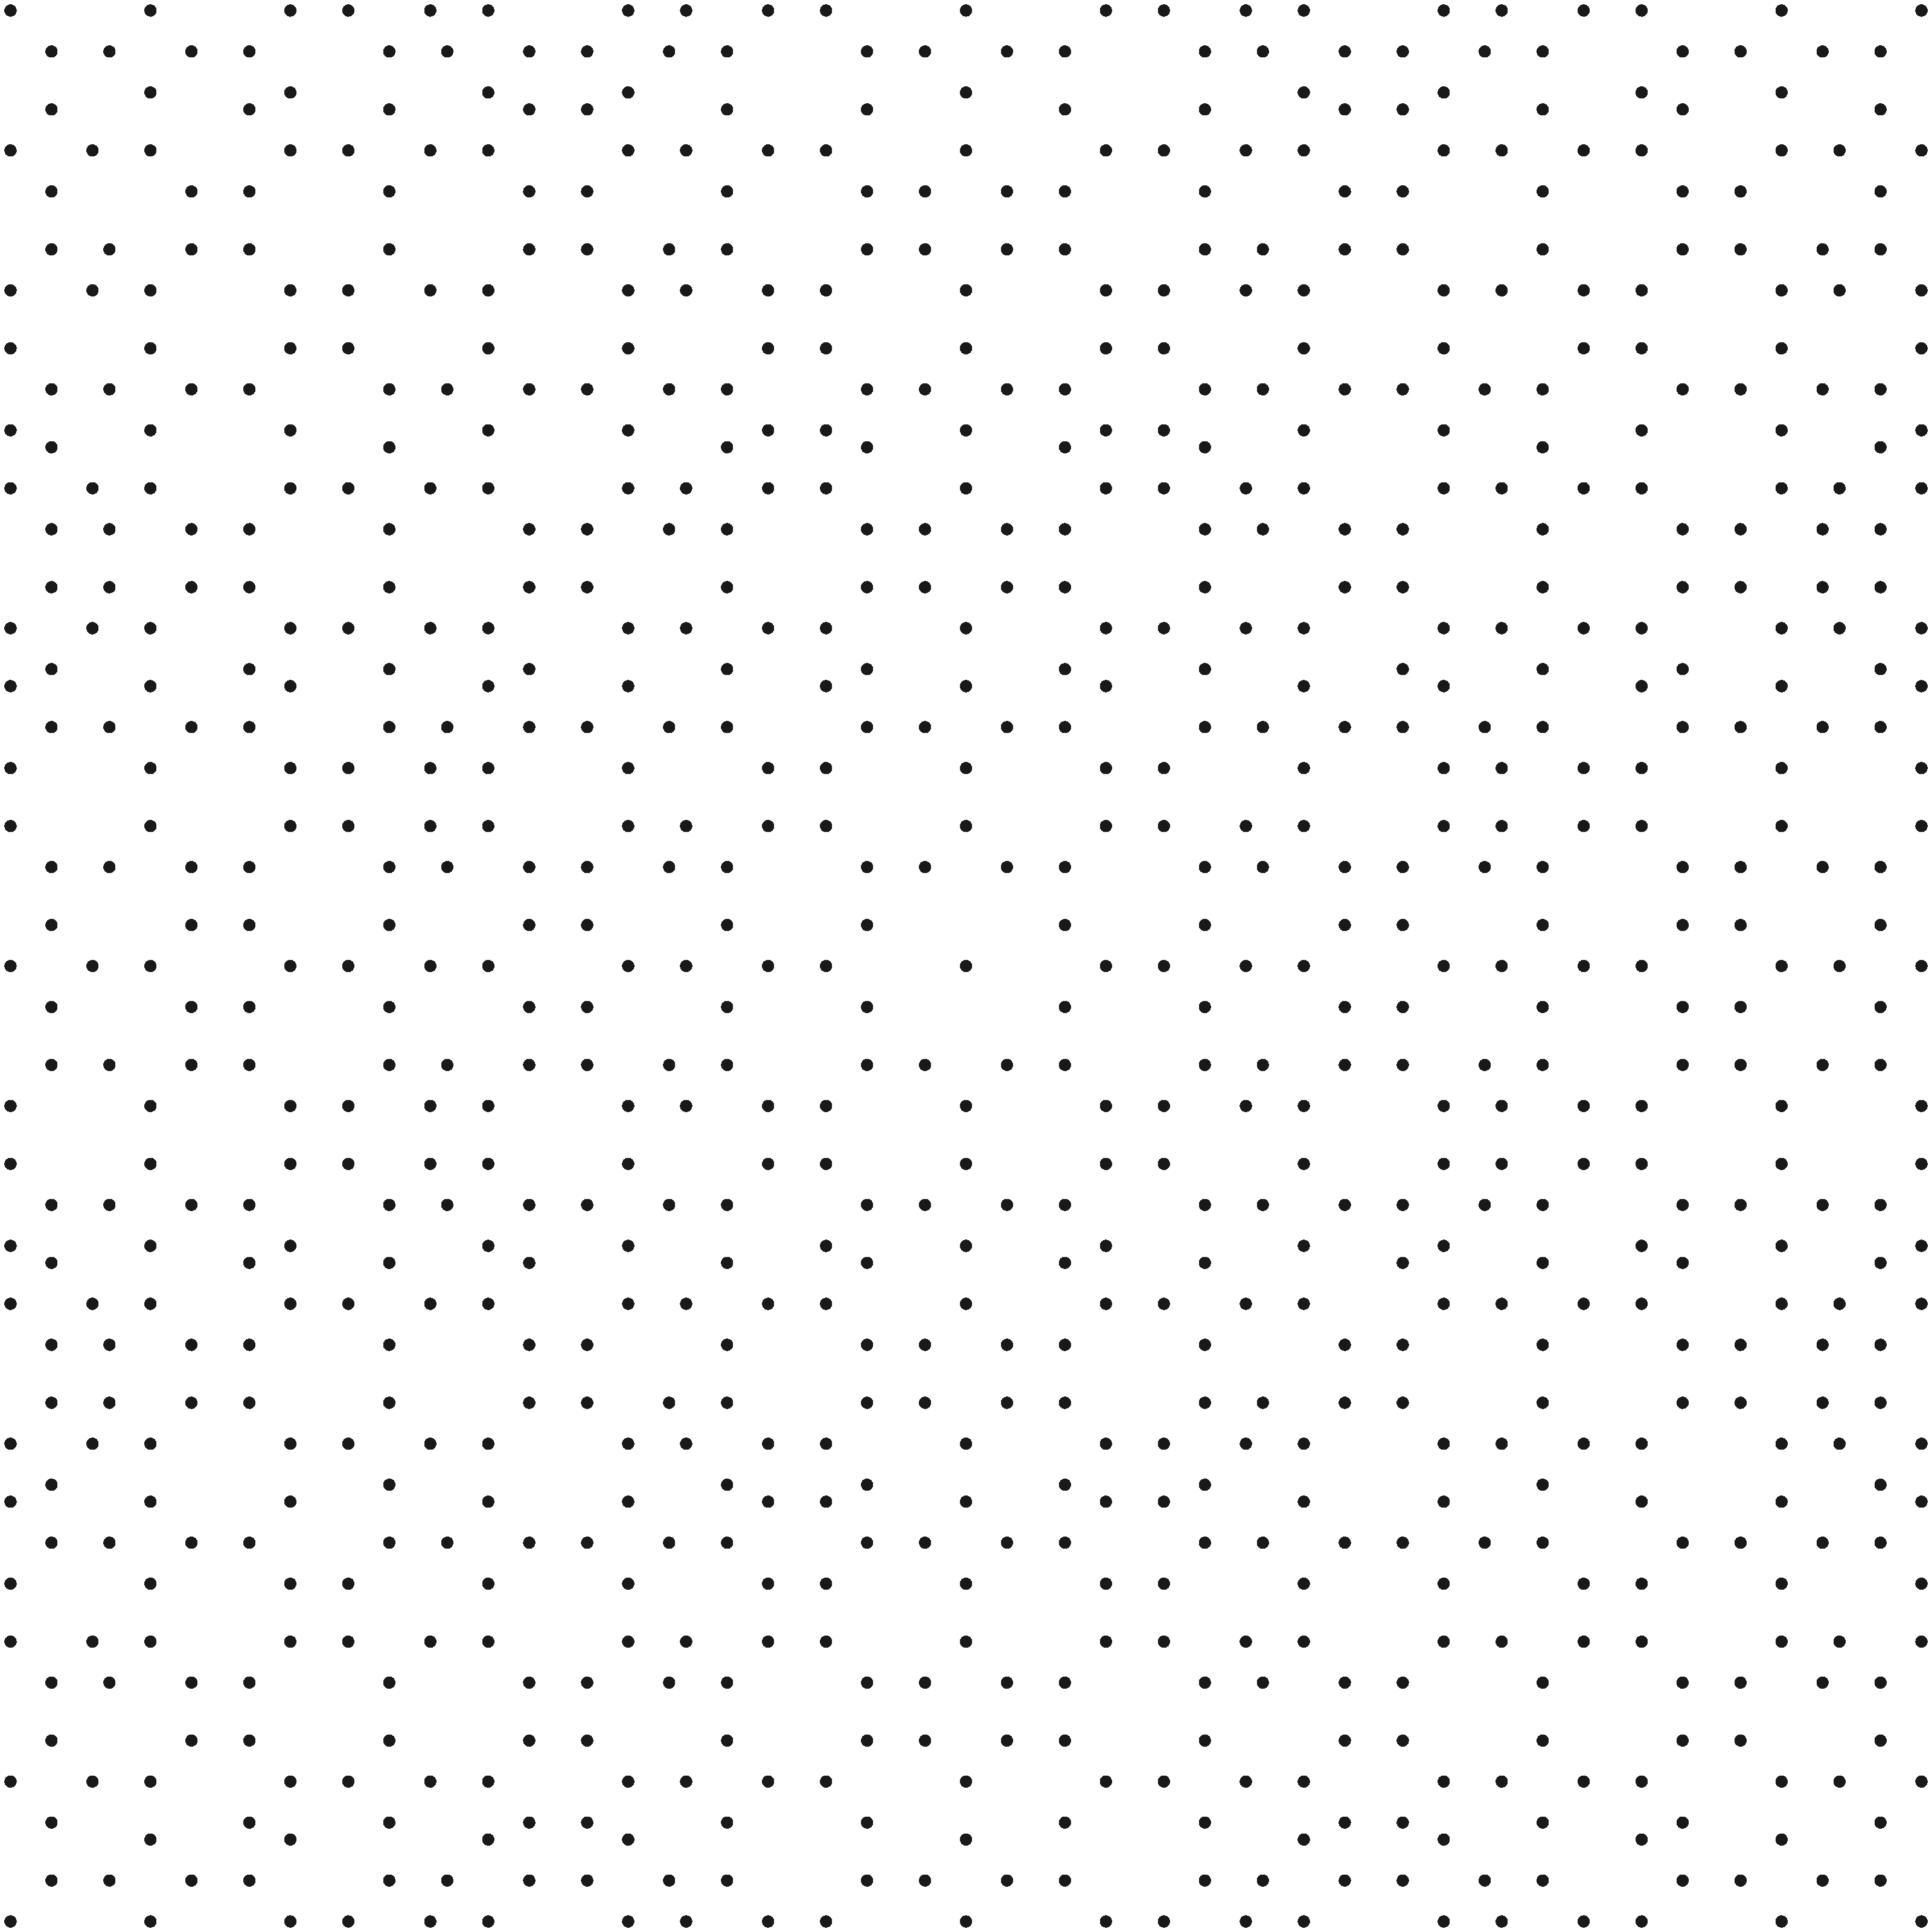
\includegraphics[width=0.9\textwidth]{img/firstExample}
\caption{Example of a two dimensional quasicrystal.}
\label{fig_quasicrystalFirstExample}
\end{figure}

We close this section with a list of properties of quasicrystals which are crucial for our analysis but also very obvious from the definition. 

\begin{itemize}
\item $\Omega_1\subset\Omega_2 \quad\Rightarrow\quad \quasi{\Omega_1}\subset\quasi{\Omega_2}$
\item $\quasi{\Omega_1}\cap\quasi{\Omega_2} \quad=\quad \quasi{\Omega_1\cap\Omega_2}$
\item $\quasi{\Omega_1}\cup\quasi{\Omega_2} \quad=\quad \quasi{\Omega_1\cup\Omega_2}$
\item $\quasi{\Omega+x^\ast} \quad=\quad \quasi{\Omega}+x\qquad \text{for}\; x\in M$
%\item $\quasi{\beta\Omega} = \beta'\quasi{\Omega}$
\end{itemize}

\end{document}
